\subsection{Profil kandidata}

Kandidatu se nakon uspešne prijave otvara profil. Prikaz profila kandidata je na slici \ref{fig:profil}. 
Kandidat sa leve strane može da otvori stranicu za teorijski ispit, praktični ispit, teorijsku nastavu, praktičnu nastavu, 
može da vidi svoje uplate i da pročita neke dodatne informacije. Takođe, kandidat ima karticu za izbor grupe, za izbor termina ispita i za zakazivanje časova.

\begin{figure}[H]
  \begin{center}
      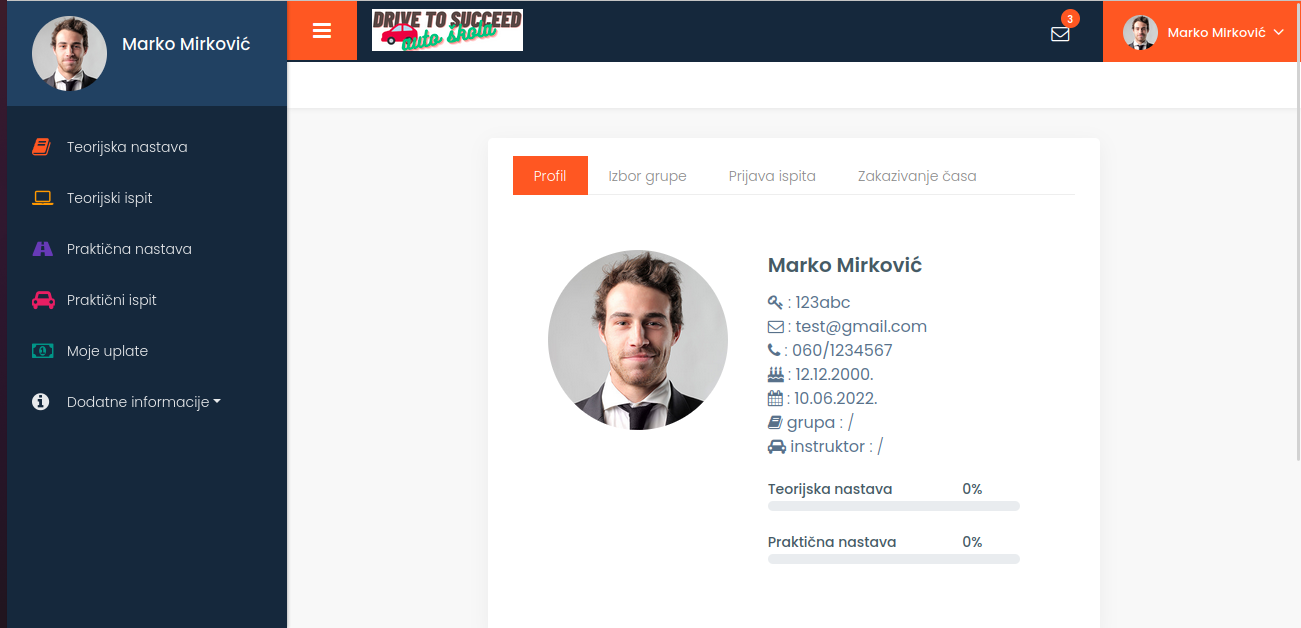
\includegraphics[width=140mm, height=60mm]{UI/UI_profil_kandidata.png}
  \end{center}
  \caption {Profil kandidata}
  \label{fig:profil}

\end{figure}

\subsection{Izbor grupe}

Kandidatu se u kartici "Izbor grupe" prikazuje lista slobodnih grupa, instruktor koji drži teorijsku obuku u toj grupi i datum početka nastave. 


Prikaz izgleda stranice za izbor grupe je dat na slici \ref{fig:ui_izbor_grupe}

\begin{figure}[H]
  \begin{center}
      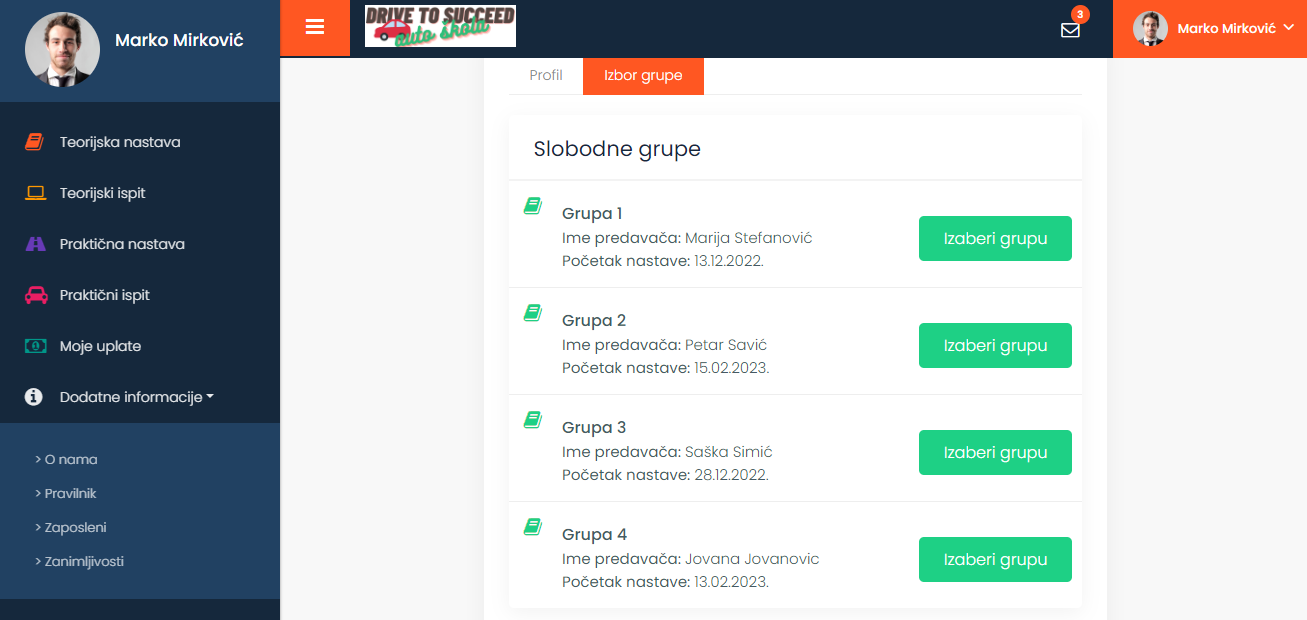
\includegraphics[width=140mm, height=60mm]{UI/UI_izbor_grupe.png}
  \end{center}
  \caption {Izbor grupe}
  \label{fig:ui_izbor_grupe}

\end{figure}

\subsection{Prijavljivanje ispita}

Kandidat nakon što je završio sa teorijskom obukom, a kasnije i sa praktičnom, može da prijavi ispit. 
Na slici \ref{fig:ui_prijava_uspesna} je prikazan izgled stranice kada kandidat ispunjava uslove za prijavu ispita. 
Prikazana je stranica za prijavu praktičnog ispita. Kandidatu su date osnovne informacije o ispitu, datum i vreme održavanja.

\begin{figure}[H]
  \begin{center}
      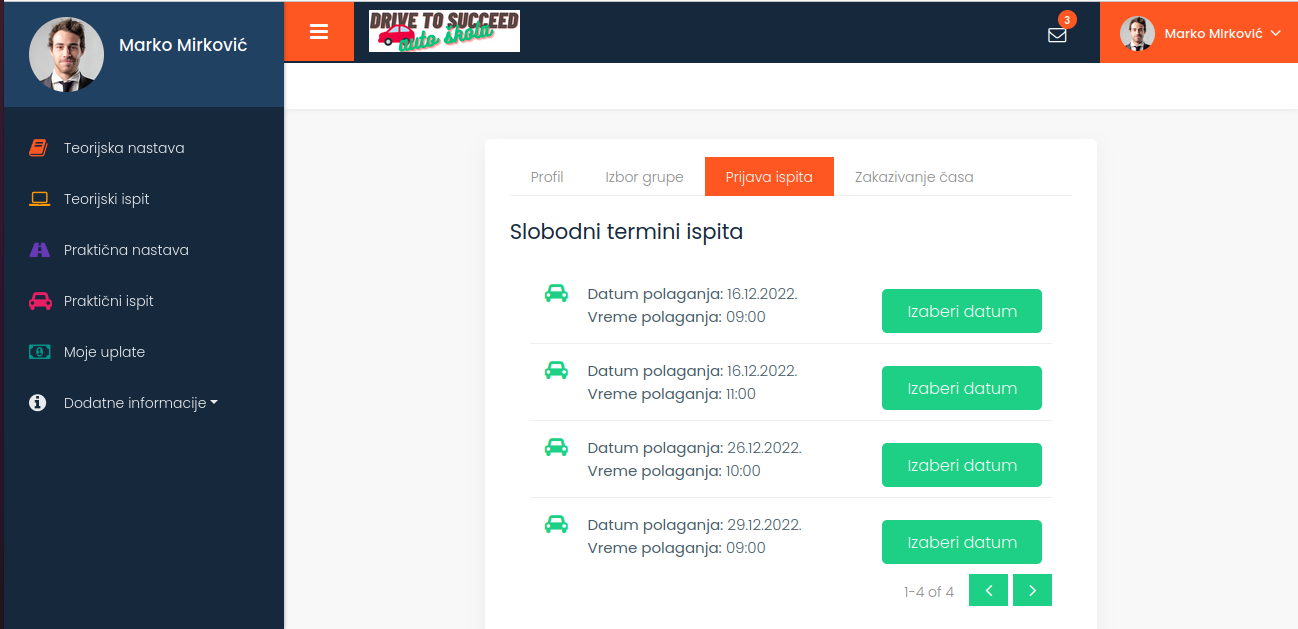
\includegraphics[width=140mm, height=60mm]{UI/UI_prijava_ispita.png}
  \end{center}
  \caption {Prijava ispita}
  \label{fig:ui_prijava_uspesna}

\end{figure}


Ako kanidat želi da prijavi ispit, a nije ispunio sve uslove za prijavu, ili trenutno nema slobodnih termina za ispit, prikazuje se poruka da trenutno nema 
slobodnih termina za ispit. Prikaz stranice je na slici \ref{fig:ui_prijava2}.

\begin{figure}[H]
  \begin{center}
      
\includegraphics[width=140mm, height=60mm]{UI/UI_prijava_ispita2.png}
  \end{center}
  \caption {Izbor grupe}
  \label{fig:ui_prijava2}

\end{figure}
